\newpage
\section{Постановка задачи}
\subsection{Назначение и общий вид манипулятора}
Целью данной курсовой работы ставится проектирование одного из двух
приводов манипулятора, устанавливаемых на малых спутниках съемки Земли (рис. \ref{sattelite_general_view}).
Манипулятор представляет собой двухзвенный электроприводной механизм,
предназначенный для скоростного наведения оптических камер.
Задачей манипулятора является организация перенацеливания камеры в заданное положение.

\begin{figure}[h!]
    \centering
    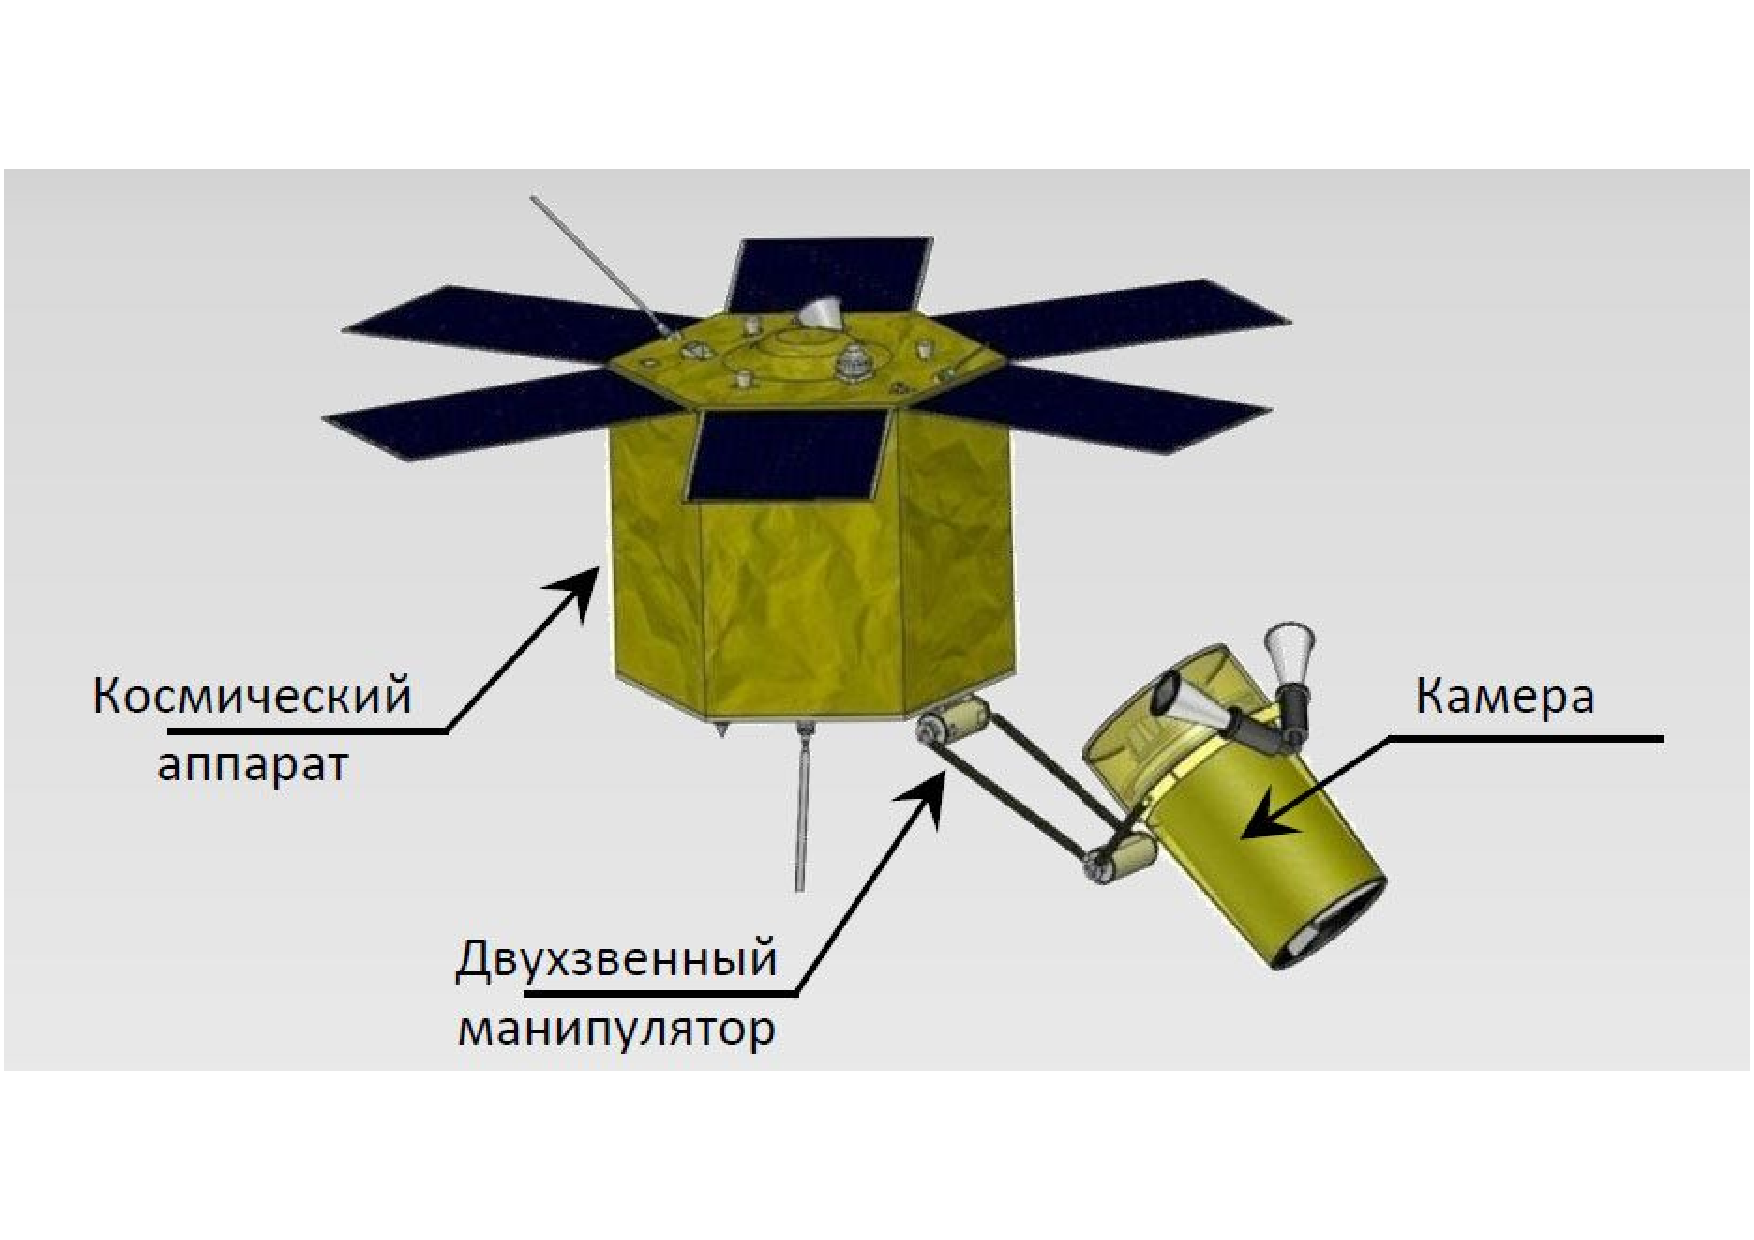
\includegraphics[width=\textwidth, keepaspectratio]{./src/pictures/sattelite_3d_images/general_view}
    \caption{Манипулятор наведения камеры малого КА}
    \label{sattelite_general_view}
\end{figure}

Программные движения манипулятора осуществляются с помощью двух электроприводных блоков,
обеспечивающих поворот камеры в одной плоскости (в плоскости перпендикулярной
вектору движения космического аппарата по орбите).

В данный момент манипуляторы подобного рода на спутниках широко востребованы
в областях картографирования, планировки территорий, образовательных,
разведывательных и военных целях, метеорологии и т.п.

К подобным манипуляторам предъявляют высокие требования по точности,
надежности, массе, габаритам.

В качестве объекта проектирования был выбран малый привод, непосредственно вращающий камеру.

\newpage
\subsection{Описание объекта управления}
Проектируемый привод установлен на малом спутнике Земли и представляет собой
исполнительный элемент системы дистанционного зондирования Земли (далее - ДЗЗ).
Объектом управления является специальная камера (рис. \ref{control_object_general_view}), предназначенная для создания
снимком поверхности Земли высокой четкости, оборудована двумя звёздными
датчиками для ориентации в пространстве и находящаяся внутри корпуса
экранно-вакуумной теплоизоляции (далее - ЭВТИ).

\begin{figure}[h!]
    \centering
    \begin{minipage}{0.5\textwidth}
        \centering
        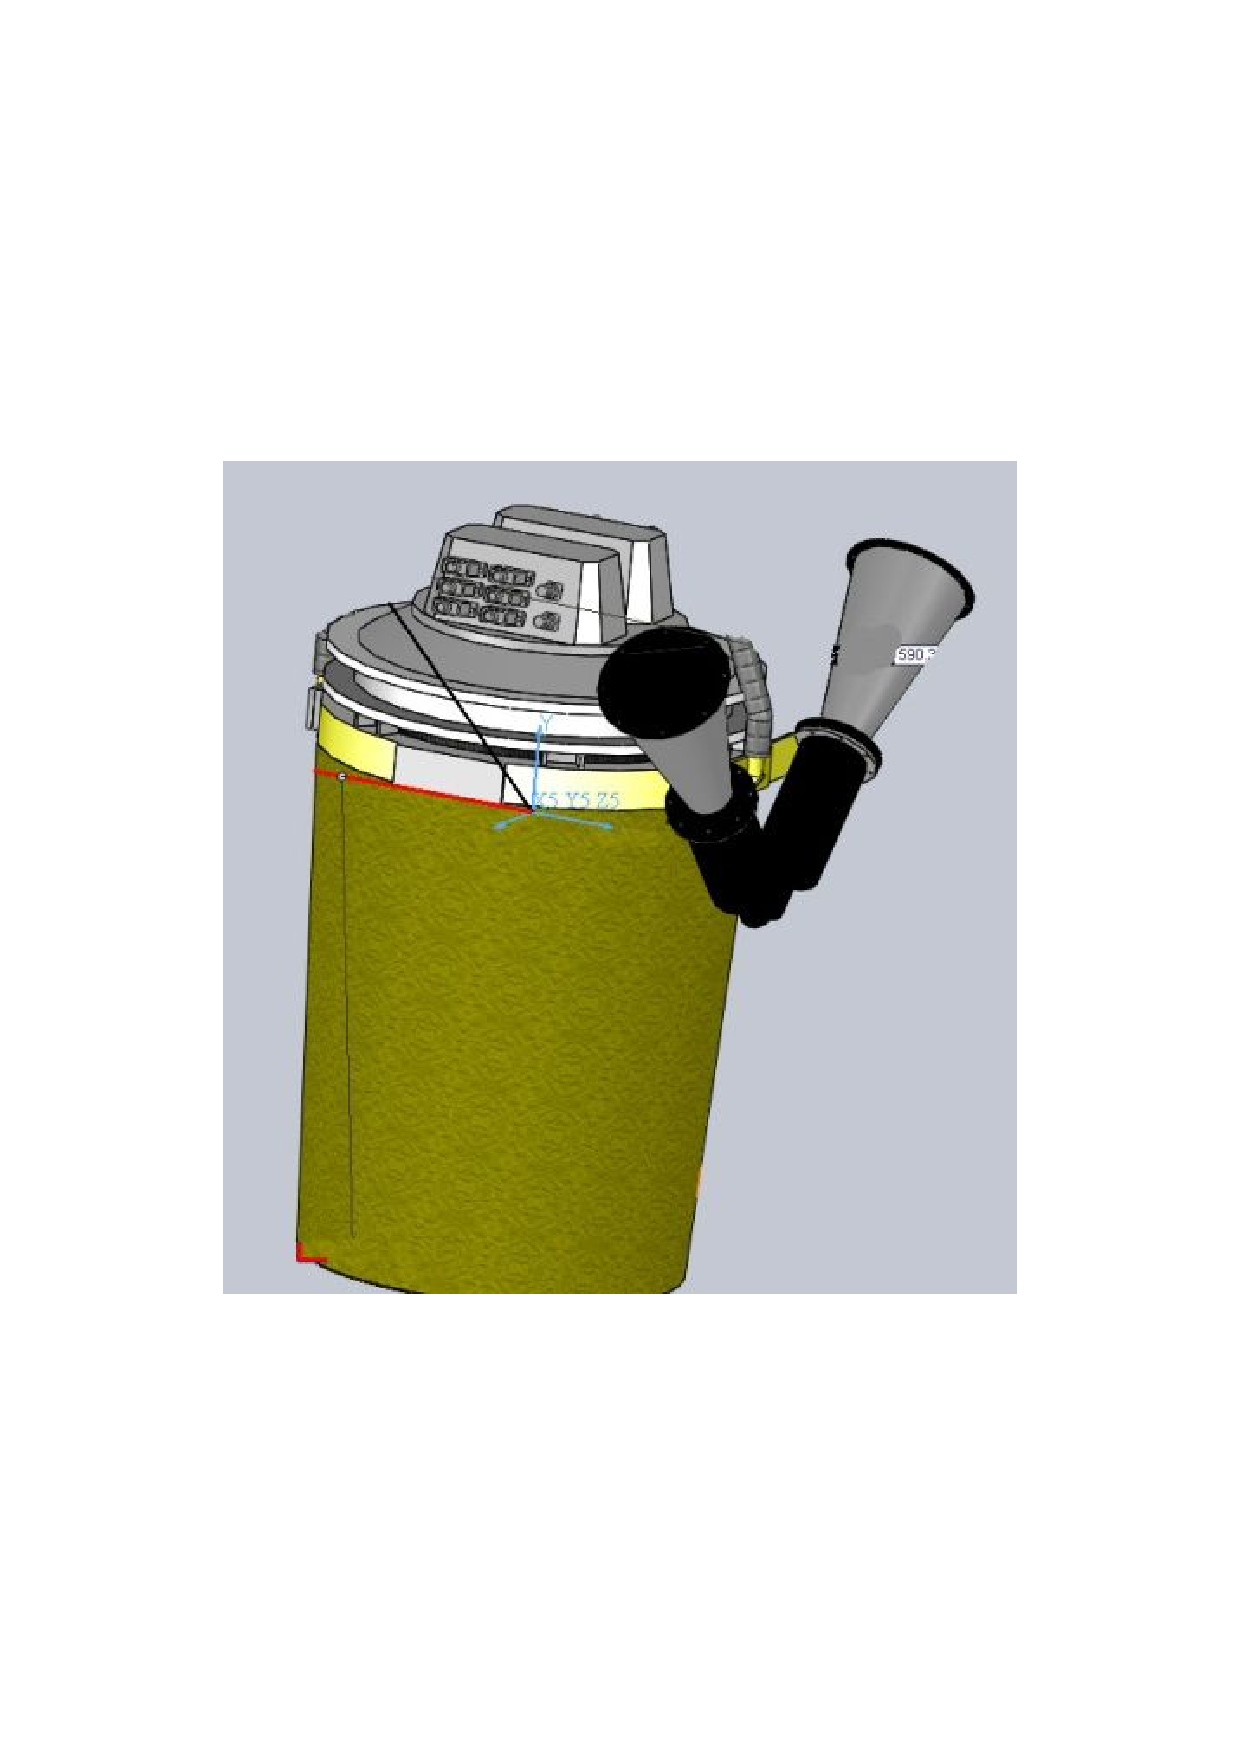
\includegraphics[width=0.5\linewidth, keepaspectratio]
                        {./src/pictures/sattelite_3d_images/control_object_view_1}
        \label{control_object_view_1}
    \end{minipage}~
    \begin{minipage}{0.5\textwidth}
        \centering
        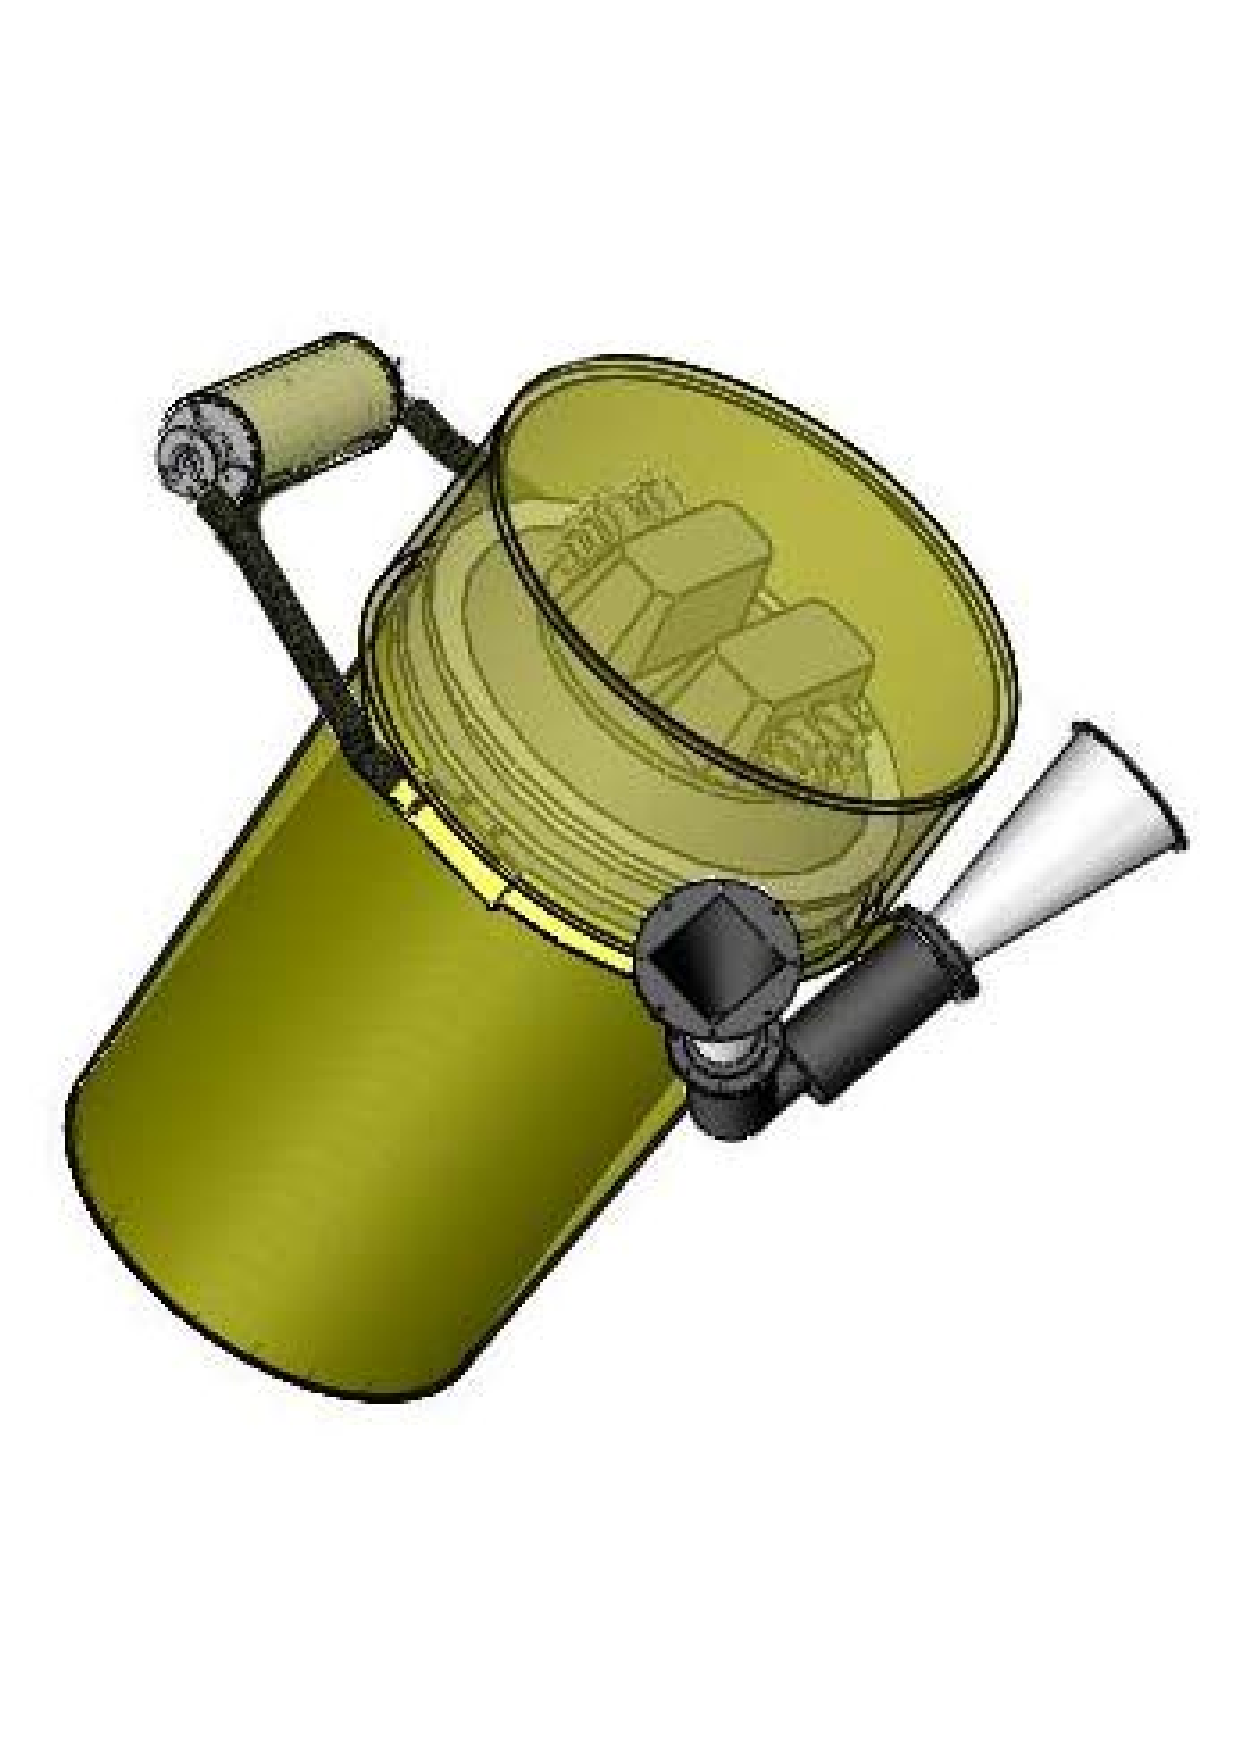
\includegraphics[width=0.5\linewidth, keepaspectratio]
                        {./src/pictures/sattelite_3d_images/control_object_view_2}
        \label{control_object_view_2}
    \end{minipage}

    \caption{Общий вид объекта управления}
    \label{control_object_general_view}
\end{figure}

\begin{table}[h!]
    \centering
    \begin{tabular}{|c|c|}
        \hline
            Эскиз & Описание \\
        \hline
            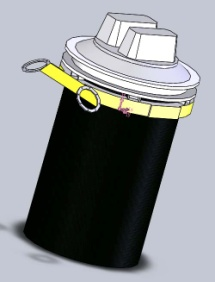
\includegraphics[height=20mm, keepaspectratio]
                            {./src/pictures/sattelite_3d_images/camera} &
            \shortstack[l] {
                \rule{0pt}{2mm} \\
                \textbf{Камера ДЗЗ:} \\
                Момент инерции вокруг продольной оси: 1,22 $\text{кг} \cdot \text{м}^{2}$ \\
                Момент инерции вокруг каждой из двух поперечных  осей: 2,17 $\text{кг} \cdot \text{м}^{2}$ \\
                Масса: 49,84 кг \\
                \rule{0pt}{2mm}
            } \\
        \hline
            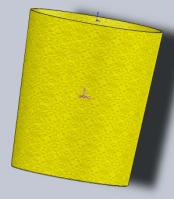
\includegraphics[height=20mm, keepaspectratio]
                            {./src/pictures/sattelite_3d_images/bottom_shell_part} &
            \shortstack[l] {
                \rule{0pt}{2mm} \\
                \textbf{Нижняя часть ЭВТИ:} \\
                Момент инерции вокруг продольной оси: 0,18 $\text{кг} \cdot \text{м}^{2}$ \\
                Момент инерции вокруг каждой из двух поперечных  осей: 0,18 $\text{кг} \cdot \text{м}^{2}$ \\
                Масса: 4,37 кг \\
                Продольная длина = 0,5 м \\
                \rule{0pt}{2mm}
            } \\
        \hline
            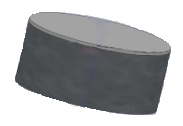
\includegraphics[height=20mm, keepaspectratio]
                            {./src/pictures/sattelite_3d_images/top_shell_part} &
            \shortstack[l] {
                \rule{0pt}{2mm} \\
                \textbf{Верхняя часть ЭВТИ:} \\
                Момент инерции вокруг продольной оси: 0,07 $\text{кг} \cdot \text{м}^{2}$ \\
                Момент инерции вокруг каждой из двух поперечных  осей: 0,04 $\text{кг} \cdot \text{м}^{2}$ \\
                Масса: 1,53 кг \\
                Продольная длина = 0,25 м \\
                \rule{0pt}{2mm}
            } \\
        \hline
            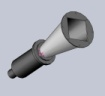
\includegraphics[height=20mm, keepaspectratio]
                            {./src/pictures/sattelite_3d_images/star_sensor} &
            \shortstack[l] {
                \rule{0pt}{2mm} \\
                \textbf{Звездный датчик (2 шт.):} \\
                Момент инерции вокруг продольной оси: 0,00 $\text{кг} \cdot \text{м}^{2}$ \\
                Момент инерции вокруг каждой из двух поперечных  осей: 0,02 $\text{кг} \cdot \text{м}^{2}$ \\
                Масса: 2,08 кг \\
                \rule{0pt}{2mm}
            } \\
        \hline
            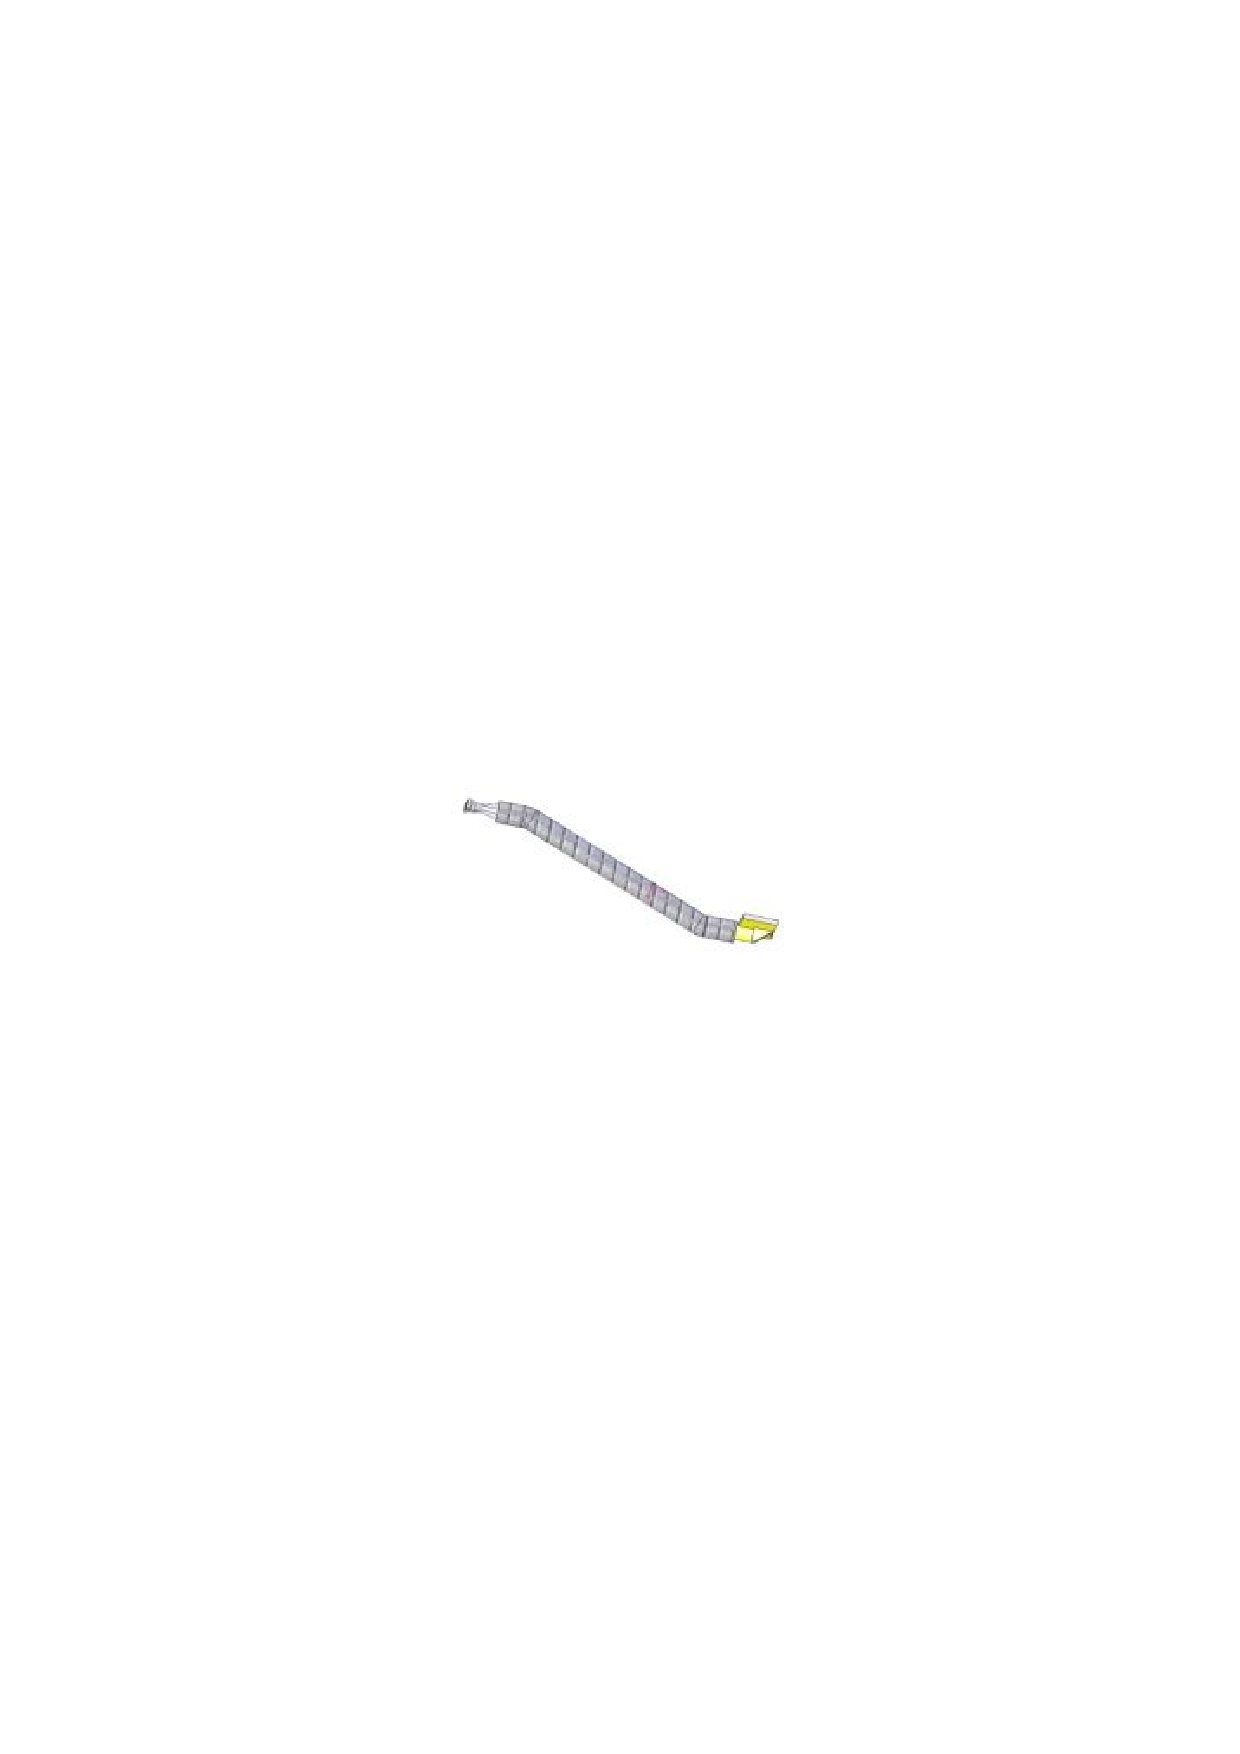
\includegraphics[height=20mm, keepaspectratio]
                            {./src/pictures/sattelite_3d_images/sleeve} &
            \shortstack[l] {
                \rule{0pt}{2mm} \\
                \textbf{Рукав (2 шт.):} \\
                Момент инерции вокруг продольной оси: 0,00 $\text{кг} \cdot \text{м}^{2}$ \\
                Момент инерции вокруг каждой из двух поперечных  осей: 0,02 $\text{кг} \cdot \text{м}^{2}$ \\
                Масса: 0,3 кг \\
                \rule{0pt}{2mm}
            } \\
        \hline
    \end{tabular}

    \caption{Составные элементы объекта управления}
\end{table}

Общая масса камеры и ее навесных элементов: $60.5 ~\text{кг}$. С учетом запаса, выберем
массу объекта управления манипулятора: $80 ~\text{кг}$.
Расстояние от оси привода до центра масс камеры: $400 ~\text{мм}$ (с учетом запаса
на более габаритную камеру и запаса на ускорение камеры);
Собственный момент инерции объекта управления вокруг оси, параллельной оси привода:
$ J_{\text{ОУ}} = 2.84 ~\text{кг} \cdot \text{м}^2 $

Момент инерции объекта управления относительно оси привода:
$ J = 15.7 ~\text{кг} \cdot \text{м}^2 $

\textit{Примечание:} полученная величина момента инерции объекта управления относительно
оси привода 2 соответствует величине, вычисленной с помощью программы SolidWorks.

\subfile{src/drive_parameters}

\endinput

